\documentclass[20]{beamer}

\usetheme{Boadilla}
\definecolor{c}{rgb}{0,0,.25}
\usecolortheme[named=c]{structure}
\usefonttheme{structureitalicserif}

\usepackage[ngerman]{babel}
\usepackage[utf8]{inputenc}
\usepackage[T1]{fontenc} 
\usepackage{graphicx}
\usepackage{feynmp-auto}
\usepackage{hyperref}
\usepackage{listings}
\usepackage{ragged2e}
\usepackage{etoolbox}
\usepackage{adjustbox}
\usepackage{pythontex}
\apptocmd{\frame}{}{\justifying}{}

\newenvironment{variableblock}[3]{%
  \setbeamercolor{block body}{#2}
  \setbeamercolor{block title}{#3}
  \begin{block}{#1}}{\end{block}}

\title[ACMA]{\textbf{Python - Funciones y Clases}}
\author[Juan David]{
\textbf{Autor:}\\
Juan David Argüello Plata - Ingeniero Mecánico\\
\vspace{5pt}
\textbf{Profesor tutor:}\\
Jairo René Martínez Morales - Químico PhD
}
\institute[]{
	CENIVAM\\
	Universidad Industrial de Santander
}
\date{}

\begin{document}

\begin{frame}
\titlepage
\end{frame}

\begin{frame}[t]{Introducción}\vspace{10pt}

\begin{figure}
\centering

\includegraphics[width=0.6\textwidth]{Images/sqlite.PNG}
\end{figure}

Una base de datos es un \textbf{sistema de almacenamiento} de información. Es como una especie de ``Excel binario`` (lenguaje SQL $\rightarrow$ ``Structured Query Language``). La información se organiza en tablas que puede llegar a tener cierto nivel de \textit{protección} contra hackers.

\vspace{5pt}

En pocas palabras: ya sabemos cómo crear datos... \textbf{ahora aprenderemos cómo almacenarlos}.

\end{frame}
\begin{frame}[t]{Objetivos}\vspace{10pt}

Los objetivos de hoy...

\begin{itemize}
	\item Instalar y conocer la interfaz de Jupyter lab.
	\item Bases de \LaTeX y HTML.
	\item Primer acercamiento a \textit{Sympy}.
	\item Enlazar clases en la interfaz de Jupyter.
	\item Desarrollar gr\'aficas en Matplotlib.
\end{itemize}

\end{frame}
\begin{frame}[fragile]{Funciones}\vspace{10pt}

Una \textit{funci\'on} es un segmento de c\'odigo que desarrolla una tarea espec\'ifica. Las funciones se escriben com\'unmente al principio o al final del \textit{Sketch}, o \textit{Script}, y se \textbf{llaman} dentro de otras funciones.

\vspace{5pt}

Las ventajas de usar funciones son:

\begin{itemize}
	\item Ayudan a mantener la \textbf{organizaci\'on} del c\'odigo (conceptualiza el algoritmo escrito).
	\item Permiten probar ``tareas" \textbf{una sola vez}.
	\item Disminuye probabilidades de errores de programaci\'on.
	\item Permite reutilizar c\'odigo.
\end{itemize}

\begin{center}
\begin{lstlisting}
	TV nombre_funcion (TV var1, TV var2, ...) {
		...
		return resultados;	//Opcional...	
	}
\end{lstlisting}
\end{center}

\end{frame}
\begin{frame}[fragile]{Funciones - sintaxis}\vspace{10pt}

La \textbf{sintaxis} de una función es la siguiente:

\begin{center}
\begin{lstlisting}
	def <nombre func> (<entradas>):
		<algoritmo>
		return salidas	(opcional)
\end{lstlisting}
\end{center}

Por ejemplo: una función de suma de dos números sería algo como:

\begin{center}
\begin{lstlisting}
	def suma (a,b):
		return a+b
	
	if __name__ == '__main__':
		print(suma(2,3))
\end{lstlisting}
\end{center}

\end{frame}
\begin{frame}[t]{Funciones - Ejercicio}\vspace{10pt}

Desarrolla los siguientes ejercicios:

\begin{itemize}
	\item Define una función que identifique si un número es par o impar.
	\item Las siguientes personas desean ingresar a un bar:
	\begin{table}[h!]
\begin{tabular}{|l|r|}
\hline
\multicolumn{1}{|c|}{\textbf{Persona}} & \multicolumn{1}{c|}{\textbf{Edad}} \\ \hline
Juan                                   & 26            \\ \hline
Sebasti\'an                              & 14                                 \\ \hline
Ramiro                                 & 22                                 \\ \hline
Mar\'ia                                  & 16                                 \\ \hline
Fabi\'an                                 & 20                                 \\ \hline
Diego                                 & 17                                \\ \hline
\end{tabular}
\end{table}
	Imprime una lista de quiénes pueden entrar.
	\item \textit{¿La revancha de Fibonacci?} Desarrolla un algoritmo que permita obtener la lista de números de Fibonacci en un rango aleatorio...
\end{itemize}

\end{frame}
\begin{frame}[allowframebreaks]{Clases}\vspace{0pt}

Las clases son \textit{estructuras} o algoritmos que permiten dividir un concepto complejo en conceptos simples que pueden ser tanto \underline{generales} como \underline{detallados}. Para el caso del semillero, podríamos pensar en algo como esto:

\begin{figure}
	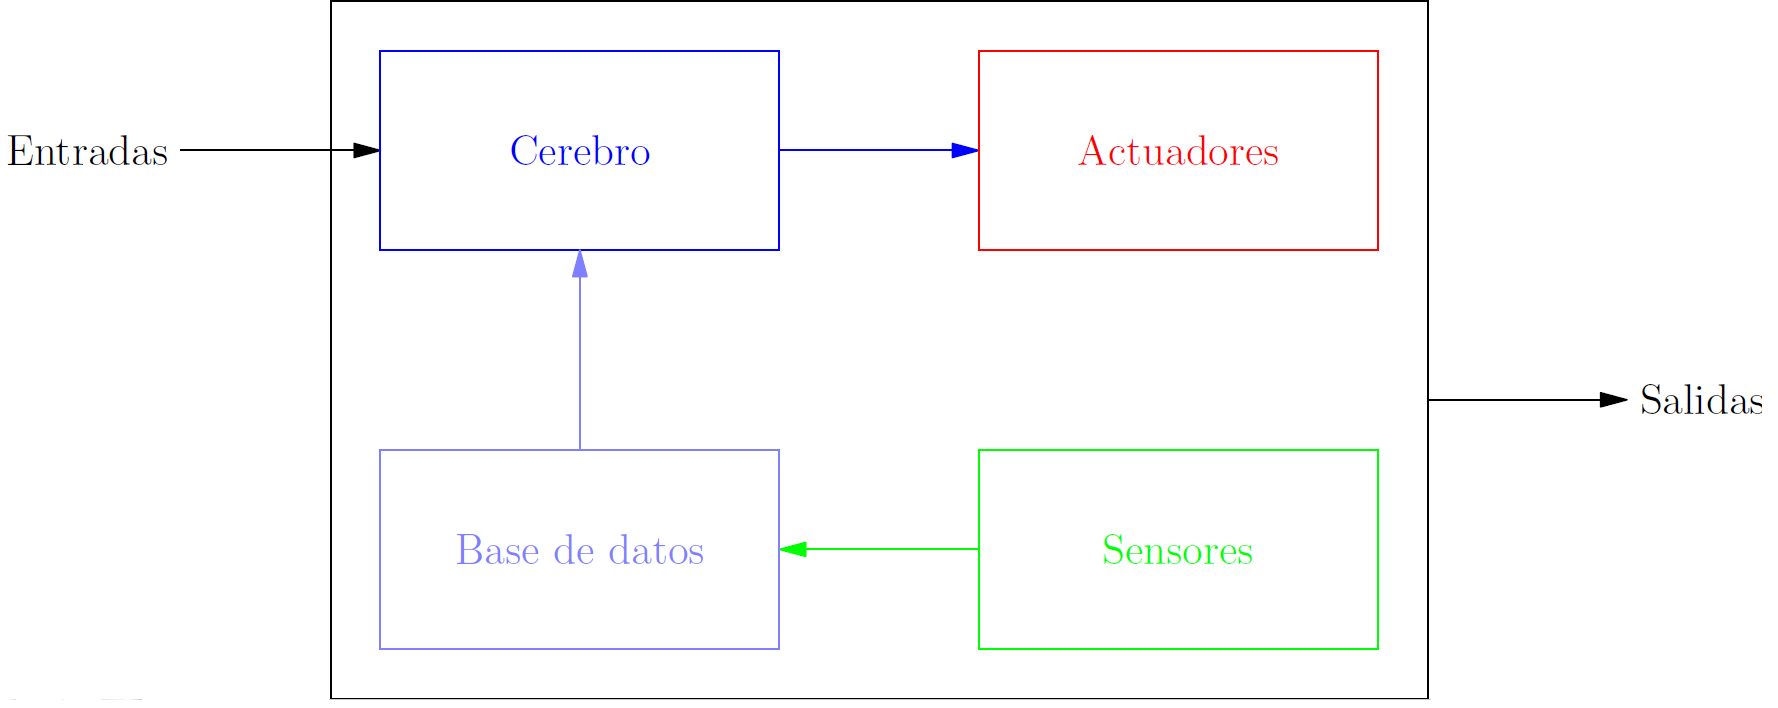
\includegraphics[scale=0.35]{Images/Esquema/Esquema.PNG}
\end{figure}

\vspace{30pt}

Las \textbf{entradas} del sistema son:

\begin{itemize}
	\item Tipo de cultivo.
	\item Ubicación de plantas.
	\item Fecha de desarrollo.
\end{itemize}

Las \textbf{salidas} son:

\begin{itemize}
	\item Cantidad de producto.
	\item Datos recolectados durante el desarrollo.
\end{itemize}

\end{frame}
\begin{frame}[fragile]{Clases - sintaxis}\vspace{0pt}

La sintaxis más básica es la siguiente:

\begin{center}
\begin{lstlisting}
	class <Nombre de la clase>:
		...
\end{lstlisting}
\end{center}

La sintaxis \underline{más completa}:

\begin{center}
\begin{lstlisting}
class <Nombre de la clase> (<Clase padre>):
  <Propiedades generales>
  def __init__(self, <entradas>):
    (...)
    super().__init__(<entr. padre>)	(OPCIONAL)
	
  def <nombre func. interna> (self, <entradas>):
    (...)
    return salidas	(OPCIONAL)
  
  def __call__(self):
  	return <resultados>
\end{lstlisting}
\end{center}

\end{frame}
\begin{frame}[fragile]{Clases - sintaxis}\vspace{0pt}

\begin{enumerate}
	\item ``def \_\_init\_\_ (self, <entradas>)": corresponde al algoritmo que se inicializará el momento en que se \underline{llame} a una clase (una clase es llamada de la misma manera que una función: ``ClassName()``). 
	\item ``super().\_\_init\_\_(<entr. padre>)``: llama la funci\'on \textit{def \_\_init\_\_} de la clase \textbf{padre}.
	\item ``def <nombre func. interna> (self, ...)``: se conocen como \textit{m\'etodos} de la clase. Se pueden llamar por fuera de la misma. Por ejemplo: tenemos una clase llamada ``Alumno``, y uno de sus m\'etodos es ``horario``. Se llamaría: Alumno.horario(<entradas del método>).
	\item ``def \_\_call\_\_ (self)``: permite obtener resultados de las clases. Cuando las clases son llamadas desde \textit{afuera}, se convierten en \textbf{objetos}. NO podemos obtener informaci\'on \'util de objetos a menos que los ``llamemos``. Se invoca la funci\'on \textit{call} poniendo un par\'entesis al final; por ejemplo: Juan = Alumno() $\rightarrow$ nos da un objeto. pero Juan(), nos da los resultados de la clase. 
\end{enumerate}

\end{frame}
\begin{frame}[allowframebreaks]{Librer\'ias}\vspace{10pt}

Python es reconocido como el lenguaje por defecto de la \textit{ciencia de datos}. En parte se debe a las librer\'ias disponibles.

\begin{block}{Instalar una librer\'ia...}
	pip install <nombre de la libreria>
\end{block}

\begin{figure}
	
\includegraphics[scale=0.5]{Images/lib.png}
\end{figure}

\begin{figure}
	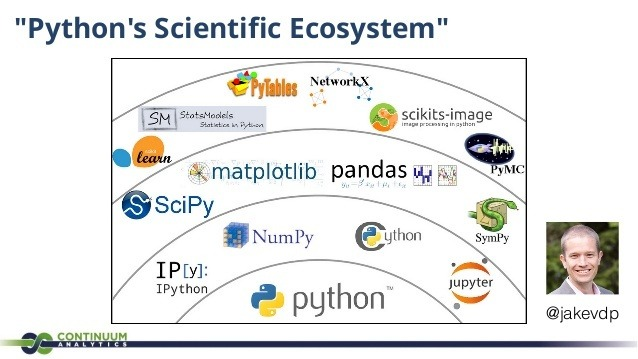
\includegraphics[scale=0.65]{Images/ecosystem.jpg}
\end{figure}

\end{frame}
\end{document}
